\documentclass{tufte-book}
\usepackage{minted}
\usemintedstyle{solarized}
\definecolor{bg}{RGB}{253,246,227}
\newminted{java}{bgcolor=bg,frame=lines,framesep=2mm}
\newminted{xml}{bgcolor=bg,frame=lines,framesep=2mm}
\newminted{python}{bgcolor=bg,frame=lines,framesep=2mm}
\hypersetup{colorlinks}

%%
% Book metadata
\title{Using Biological Pathway Data with Paxtools: A User's Guide}

\author[Paxtools Developers]{Paxtools Developers}


%%
% For nicely typeset tabular material
\usepackage{booktabs}

%%
% For graphics / images
\usepackage{graphicx}
\setkeys{Gin}{width=\linewidth,totalheight=\textheight,keepaspectratio}
\graphicspath{{graphics/}}

% The fancyvrb package lets us customize the formatting of verbatim
% environments. We use a slightly smaller font.
\usepackage{fancyvrb}
\fvset{fontsize=\normalsize}

%%
% Prints argument within hanging parentheses (i.e., parentheses that take
% up no horizontal space). Useful in tabular environments.
\newcommand{\hangp}[1]{\makebox[0pt][r]{(}#1\makebox[0pt][l]{)}}

%%
% Prints an asterisk that takes up no horizontal space.
% Useful in tabular environments.
\newcommand{\hangstar}{\makebox[0pt][l]{*}}

%%
% Prints a trailing space in a smart way.
\usepackage{xspace}


\newcommand{\TL}{Tufte-\LaTeX\xspace}

% Prints the month name (e.g., January) and the year (e.g., 2008)
\newcommand{\monthyear}{%
\ifcase\month\or January\or February\or March\or April\or May\or June\or
July\or August\or September\or October\or November\or
December\fi\space\number\year
}



% Inserts a blank page
\newcommand{\blankpage}{\newpage\hbox{}\thispagestyle{empty}\newpage}

\usepackage{units}

% Typesets the font size, leading, and measure in the form of 10/12x26 pc.
\newcommand{\measure}[3]{#1/#2$\times$\unit[#3]{pc}}

% Macros for typesetting the documentation
\newcommand{\hlred}[1]{\textcolor{Maroon}{#1}}% prints in red
\newcommand{\hangleft}[1]{\makebox[0pt][r]{#1}}
\newcommand{\hairsp}{\hspace{1pt}}% hair space
\newcommand{\hquad}{\hskip0.5em\relax}% half quad space
\newcommand{\TODO}{\textcolor{red}{\bf TODO!}\xspace}
\newcommand{\ie}{\textit{i.\hairsp{}e.}\xspace}
\newcommand{\eg}{\textit{e.\hairsp{}g.}\xspace}
\newcommand{\na}{\quad--}% used in tables for N/A cells
\providecommand{\XeLaTeX}{X\lower.5ex\hbox{\kern-0.15em\reflectbox{E}}\kern-0.1em\LaTeX}
\newcommand{\tXeLaTeX}{\XeLaTeX\index{XeLaTeX@\protect\XeLaTeX}}
% \index{\texttt{\textbackslash xyz}@\hangleft{\texttt{\textbackslash}}\texttt{xyz}}
\newcommand{\tuftebs}{\symbol{'134}}% a backslash in tt type in OT1/T1
\newcommand{\doccmdnoindex}[2][]{\texttt{\tuftebs#2}}% command name -- adds backslash automatically (and doesn't add cmd to the index)
\newcommand{\doccmddef}[2][]{%
\hlred{\texttt{\tuftebs#2}}\label{cmd:#2}%
\ifthenelse{\isempty{#1}}%
{% add the command to the index
\index{#2 command@\protect\hangleft{\texttt{\tuftebs}}\texttt{#2}}% command name
}%
{% add the command and package to the index
\index{#2 command@\protect\hangleft{\texttt{\tuftebs}}\texttt{#2} (\texttt{#1} package)}% command name
\index{#1 package@\texttt{#1} package}\index{packages!#1@\texttt{#1}}% package name
}%
}% command name -- adds backslash automatically
\newcommand{\doccmd}[2][]{%
\texttt{\tuftebs#2}%
\ifthenelse{\isempty{#1}}%
{% add the command to the index
\index{#2 command@\protect\hangleft{\texttt{\tuftebs}}\texttt{#2}}% command name
}%
{% add the command and package to the index
\index{#2 command@\protect\hangleft{\texttt{\tuftebs}}\texttt{#2} (\texttt{#1} package)}% command name
\index{#1 package@\texttt{#1} package}\index{packages!#1@\texttt{#1}}% package name
}%
}% command name -- adds backslash automatically
\newcommand{\docopt}[1]{\ensuremath{\langle}\textrm{\textit{#1}}\ensuremath{\rangle}}% optional command argument
\newcommand{\docarg}[1]{\textrm{\textit{#1}}}% (required) command argument
\newenvironment{docspec}{\begin{quotation}\ttfamily\parskip0pt\parindent0pt\ignorespaces}{\end{quotation}}% command specification environment
\newcommand{\docenv}[1]{\texttt{#1}\index{#1 environment@\texttt{#1} environment}\index{environments!#1@\texttt{#1}}}% environment name
\newcommand{\docenvdef}[1]{\hlred{\texttt{#1}}\label{env:#1}\index{#1 environment@\texttt{#1} environment}\index{environments!#1@\texttt{#1}}}% environment name
\newcommand{\docpkg}[1]{\texttt{#1}\index{#1 package@\texttt{#1} package}\index{packages!#1@\texttt{#1}}}% package name
\newcommand{\doccls}[1]{\texttt{#1}}% document class name
\newcommand{\docclsopt}[1]{\texttt{#1}\index{#1 class option@\texttt{#1} class option}\index{class options!#1@\texttt{#1}}}% document class option name
\newcommand{\docclsoptdef}[1]{\hlred{\texttt{#1}}\label{clsopt:#1}\index{#1 class option@\texttt{#1} class option}\index{class options!#1@\texttt{#1}}}% document class option name defined
\newcommand{\docmsg}[2]{\bigskip\begin{fullwidth}\noindent\ttfamily#1\end{fullwidth}\medskip\par\noindent#2}
\newcommand{\docfilehook}[2]{\texttt{#1}\index{file hooks!#2}\index{#1@\texttt{#1}}}
\newcommand{\doccounter}[1]{\texttt{#1}\index{#1 counter@\texttt{#1} counter}}

\newenvironment{tightcenter}{%
  \setlength\topsep{0pt}
  \setlength\parskip{0pt}
  \begin{center}
}{%
  \end{center}
}

% Generates the index
\usepackage{makeidx}
\makeindex

\begin{document}

\begin{titlepage}
\begin{tightcenter}

% Upper part of the page. The '~' is needed because \\
% only works if a paragraph has started.

\textsc{\LARGE Paxtools Developers}\\[5.5cm]


% Title

{ \huge \bfseries Using Biological Pathway Data with Paxtools}\\[0.4cm]


\textsc{\Large  A User's Guide}\\[0.5cm]

\end{tightcenter}

\begin{fullwidth}
~\vfill
\thispagestyle{empty}
\setlength{\parindent}{0pt}
\setlength{\parskip}{\baselineskip}
Copyright \copyright\ \the\year\ \thanklessauthor


\par\smallcaps{biopax.org/paxtools}

\par \includegraphics[width=\linewidth/10]{by-nd.eps}  This work is licensed under a \href{http://creativecommons.org/licenses/by-nd/3.0/deed.en_US} {Creative Commons Attribution-NoDerivs 3.0 Unported License.} \index{license}
\par Based on the the tufte-latex template by Kevin Godby, Bil Kleb, and Bill Wood. 
\par \url{code.google.com/p/tufte-latex/} The template is distributed under Apache 2.0 License
\par\textit{Second Edition, \monthyear}
\end{fullwidth}
\end{titlepage}
% r.5 contents
\tableofcontents


% r.9 introduction
\cleardoublepage
\chapter*{Introduction}

Extraordinary advances in sequencing and other molecular technologies have led to a large increase in data about biological processes. The total volume of pathway data mapped by biologists and stored in databases has entered a rapid growth phase, with the number of online resources for pathways and molecular interactions increasing 70\%, from 190 in 2006 to 325 in 2010 \cite{Bader2006}. Unfortunately, most of these databases were originally developed to use their own pathway representation language, resulting in a heterogeneous set of resources that are extremely difficult to combine and use. It is therefore imperative to develop computational methods to cope with both the magnitude and fragmented nature of this rapidly expanding and exceedingly valuable pathway information.

A key component of this infrastructure is a common standard language. BioPAX (Biological Pathway Exchange) \cite{Demir2010} is an OWL(Web Ontology Language) based community developed language for representing pathway data. Software developers can use BioPAX to maximize their application's access to pathway data from different sources. Similarly pathway database providers can reach a greater number of users through BioPAX exports.

BioPAX covers a large spectrum of pathway data, including signaling and metabolic pathways as well as genetic and protein-protein interactions. Developing software that produces or consumes BioPAX can be a daunting task at first because of the large number of classes and properties that BioPAX contains. Paxtools addresses this by offering a Java API that maps OWL classes and properties to Java beans and methods that can significantly reduce software development time. 

Paxtools can help scientists to quickly access, analyze and manipulate pathway information. Developers of BioPAX exporters, visualization tools, editors or algorithms can use Paxtools to significantly reduce time spent on BioPAX. Developing applications with Paxtools also offers future flexibility and extensibility. 

%%
% Start the main matter (normal chapters)
\mainmatter


\chapter{Getting Started}
\label{ch:features}

\section{Features of Paxtools}

Historically, Paxtools was developed to provide an OWL\sidenote{\url{http://www.w3.org/TR/owl-overview/}} -Java mapping, but today it offers much more. There are utilities for quickly traversing or manipulating objects, fixing common problems or converting pathway models to different BioPAX levels or other standards and formats. There are also BioPAX JPA (Java Persistence API) mappings for persisting large BioPAX models into a database and advanced graph queries for finding biologically relevant paths between molecules. All of these are organized in a lightweight modular structure to help you embed only the portions you need within your application with minimum footprint. Here is a list of some features:

\newthought{A complete and consistent implementation of BioPAX specification:} BioPAX elements in Paxtools are plain Java beans which provide methods to access the properties described in BioPAX, and a model, acting as a container for all BioPAX elements, provides querying facilities for them. Users can either read a BioPAX model from a file or create an empty one from scratch. Methods to add new elements to a model and to remove elements from a model are also provided.

\newthought{Support for OWL properties and additional inverse links:} OWL properties can be symmetric, transitive or subtyped into other properties. These semantics can not be represented directly in an object oriented programming language. Paxtools implements these additional semantics and automatically updates the fields of objects as needed.

\newthought{Syntactic validation:} Each operation that modifies the model is internally validated by Paxtools to comply with BioPAX syntax, including RDF well-formedness, domain and range restrictions, bidirectional links, and redundancies.

\newthought{Seamless handling of different BioPAX levels:} Recently released BioPAX Level 3 introduced significant improvements to the naming and structure of the BioPAX at some cost of backwards compatibility. Paxtools supports all three BioPAX levels (1, 2 and 3) and provides facilities for upgrading older BioPAX models to Level 3, reducing the burden of working with different BioPAX levels for developers.

\newthought{Converting to and from different formats:} Paxtools can convert PSI-MI\cite{Kerrien2007} models to BioPAX Level 3. In addition, BioPAX models can be exported back to OWL and several other useful formats, including  SBGN(Systems Biology Graph Notation)\cite{Le_Novère2009}, SIF (Simple Interaction Format) and GSEA (Gene Set Enrichment Analysis)\cite{Subramanian2005}.

\newthought{Efficient traversal and editing via reflection:} Paxtools allow tools to manipulate BioPAX models without actually hard coding property and class names. This pattern considerably simplifies development of BioPAX exporters and other tools and makes it easier to extend and update them to support future changes in the BioPAX specification. PathAccessors allow XPath like querying and traversal of the object graph. 

\newthought{Direct Access to PC:} PC (Pathway Commons)\cite{Cerami2011} is a convenient point of access to biological pathways collected from public pathway databases. Pathway Commons aggregates, validates and normalizes pathway information significantly facilitating its use for biological applications. Paxtools have a built in client that allows you to access PC, run field and graph queries and obtain results as BioPAX models. 

\newthought{Advanced Graph Queries:} Paxtools offers graph queries, such as "paths-between" or "common up/downstream" that are specifically customized based on BioPAX semantics for answering common biological questions. 

\newthought{Modular and lightweight structure:} The Paxtools core module, which provides a complete implementation of BioPAX and read in/write out functionality, is a very compact library(400 kB) that can be extended as required with additional modules. Paxtools is distributed as a Maven project which allows developers to easily select just the parts of Paxtools they need in their application.

\newthought{A platform for development of BioPAX software infrastructure:} A growing BioPAX software infrastructure, available as a part of the Pathway Commons project, is directly built on top of Paxtools, including a state-of-the-art persistence system using Java Persistence API integrated with the querying facilities, an advanced validator that allows checking complex rules and best practices using an extensible framework, and a pathway alignment tool. Paxtools is also currently being used by several software tools including CellDesigner\cite{mi2011}, Cytoscape\cite{Cline2007} and ChiBE\cite{Babur2010}. 
\bigskip

\section{Modules and Package Structure}
Here is a quick overview of the modules and packages they contain:
\begin{itemize}

\item Core: Core module contains the model interfaces and their default implementation as well as some utility classes. All other modules depend on the core. Some important packages are:
	\begin{itemize}
	\item model: This package (and its subpackages) defines the model interfaces that maps to BioPAX classes. All applications should be written to these interfaces rather than the actual implementation classes.
	\item impl: Default implementation package.
	\item controller: This package contains classes that contain logic for traversing, copying and merging BioPAX elements as well as property editors.
	\end{itemize}
\item io: Simple IO package for reading/writing BioPAX files.
 \item converter: This is to convert (upgrade) BioPAX Level1, 2 to Level 3.
\item jena IO: This module contains an alternative Jena based handler for reading/writing BioPAX files.
\item query: This module contains graph queries such as shortest-path.
\item PSI-MI converter: This module converts PSI-MI 2.5 files to BioPAX Level 2 or 3.
\item Sif, GSEA and SBGN converters: These modules export BioPAX models to SIF, GSEA and SBGN (work in progress) respectively.
\end{itemize}

\section{Obtaining Paxtools}

\subsection{Release Bundles}

You can download the "Fat" jars (with dependencies) from:
	\url{http://sourceforge.net/projects/biopax/files/paxtools/}

This is a good choice to get things working now and worry about which modules to package with your application later.

Alternatively, individual modules (compiled JARs and POMs) can be obtained from the BioPAX maven repositories:
	
	\url{http://biopax.sourceforge.net/m2repo/snapshots} and 

\url{http://biopax.sourceforge.net/m2repo/releases}
for snapshots and stable releases respectively. 

Use modules to minimize the size of your application and use only the parts of Paxtools that you need. The "Core" module offers a complete implementation of BioPAX and read in/write out functionality in a very compact 400 kB package The fat jar can be as large as 16 MB most because of the Jena library and its dependencies.


\subsection{Embedding Paxtools in a maven project}

If you are already using Maven in your project, you can add Paxtools as a dependency.
Add the following lines into your pom.xml, within the repositories section:

\begin{xmlcode}
<repository>
  <id>biopax.releases</id>
  <name>BioPAX Repository at Sourceforge</name>
  <url>http://biopax.sourceforge.net/m2repo/releases/</url>
  <snapshots>
   <enabled>false</enabled>
  </snapshots>
</repository>
\end{xmlcode}

and, if you want to use the latest builds:

\begin{xmlcode}
<repository>
  <id>biopax.snapshots</id>
  <name>BioPAX Snapshots Repository at Sourceforge</name>
  <url>http://biopax.sourceforge.net/m2repo/snapshots/</url>
  <releases>
   <enabled>false</enabled>
  </releases>
 </repository>
\end{xmlcode}

Then, add the modules of your choice in the <dependencies> element:

\begin{xmlcode}
<dependency>
  <groupId>org.biopax.paxtools</groupId>
  <artifactId>paxtools-core</artifactId>
  <version>4.1.5</version>
 </dependency>
\end{xmlcode}


\subsection{Downloading sources}

Checkout (read-only) using the Mercurial client:

\begin{fullwidth}
\begin{xmlcode}
hg clone http://biopax.hg.sourceforge.net:8000/hgroot/biopax/paxtools
\end{xmlcode}
\end{fullwidth}
More information on how to access to the source code can be found here: 	

\url{http://biopax.sourceforge.net/paxtools/source-repository.html}

\subsection{Documentation and Help}
More information on Paxtools can be found at:
\begin{fullwidth}
\begin{itemize}
\item Wiki: \url{http://sourceforge.net/apps/mediawiki/biopax/index.php?title=Paxtools} 

\item API: \url{http://www.biopax.org/m2site/}

\item If you get stuck or have questions, use Paxtools support mailing list: 	

\url{biopax-paxtools@lists.sourceforge.net}

\url{http://lists.sourceforge.net/lists/listinfo/biopax-paxtools}


\item For general questions related to BioPAX, use BioPAX discuss mailing list: 

\url{http://groups.google.com/group/biopax-discuss}

\end{itemize}
\end{fullwidth}


\chapter{Paxtools Basics}

\section{First Model}

In order to create paxtools objects, we will need a factory. For most use cases, the default factory is a good choice. We can get a level 3 specific factory by\sidenote{Paxtools supports all 3 levels of BioPAX and can upgrade previous levels to level 3. Default values are always set to level 3. We will also use level 3 for the code examples in this guide.}:

\begin{javacode}
BioPAXFactory factory = BioPAXLevel.L3.getDefaultFactory();
\end{javacode}

BioPAXLevel is an enum that contains multiple level specific facilities and fields. These can be very useful if you want to implement level agnostic facilities. You can find more information about BioPAXLevel in the API documentation.

A Paxtools model is a container for your objects. When you read, write or pass around BioPAX objects, these objects will be contained inside a model. This is useful for validation and querying purposes. 
Let's begin by creating a new model:


\begin{javacode}
Model model = factory.createModel();
\end{javacode}

Set xml:base \sidenote {OWL uses declared namespaces to make the ontology files more readable and avoid namespace clashes. Paxtools always uses full (absolute) RDF Ids for objects internally but will output relative Ids where possible when writing out BioPAX files if xml:base (URI prefix) is declared. You can reach a model's xml base using getXmlBase, setXmlBase and - namespaces using getNameSpacePrefixMap methods.}:

\begin{javacode}
model.setXmlBase("http://biopax.org/tutorial/");
\end{javacode}

Now we can create new BioPAX objects and insert them into the model:

\begin{javacode}
Protein protein1 = model.addNew(Protein.class, 
	"http://biopax.org/tutorial/test1"); 
\end{javacode}

This method will create a new instance of protein class and insert it into the model. The second parameter is a unique identifier for the  protein state. \sidenote{BioPAX uses RDF-IDs to uniquely identify resources. IDs should be valid URIs and globally unique. The best practice accepted by the BioPAX community is to use standard URI spaces, such as identifiers.org, especially for objects that map one-to-one to existing common bioinformatics resources. For example, you can refer to a uniprot ProteinReference with \url{http://identifiers.org/uniprot/P04150}. If you are planning to distribute your BioPAX models publicly consider obtaining your identifiers.org subspace and use that for assigning ids to the objects that you create, e.g. reactions or protein complexes.} You can always access an object if you know their id by the model's getByID method:

\begin{javacode}
Protein retrievedProtein = model.getByID(
	"http://biopax.org/tutorial/test1"); 
\end{javacode}






\section{Modifying Objects}

In the model package you will find interfaces for each class in BioPAX. All setter/getter methods for BioPAX properties in those interfaces follow the default java bean pattern - for single cardinality property TTT, there are two methods: setTTT/getTTT\sidenote{Unlike Object Oriented languages like Java, in OWL properties are first class citizens that can have inheritance and attributes like transitive and functional. Paxtools implements these additional semantics internally. For example, since property "standardName" is a subproperty of "name", updating the standardName of a protein will also update its list of names. }. For  multi-cardinality objects, Paxtools keeps a Set of objects. Two additional methods, addTTT and removeTTT are provided for manipulating the content of these sets.

Let's modify the fields of our newly minted protein :

\begin{javacode}
protein1.addName("Tutorial Example Some Transporter 1");
protein1.setDisplayName("TEST1");
\end{javacode}

Let's add a biochemical reaction and connect it to our protein:


\begin{javacode}
BiochemicalReaction rxn1 = model.addNew(
	BiochemicalReaction.class,
         "http://biopax.org/tutorial/rxn1");
rxn1.addLeft(protein1);
\end{javacode}

You can keep adding different properties and classes to get a complete pathway. \sidenote{In the BioPAX specification properties are unidirectional for brevity. For example, the "participant" property links interactions to physical entities. You should always add/removes properties in that "forward' direction. Paxtools also provides additional "inverse" links for key properties that allow efficient bidirectional navigation. These inverse links are also automatically updated when you modify the forward direction}.


\section{Reading and Writing BioPAX }

Most of the time you, will not be creating your model from the scratch but rather reading it from a file. For reading files, Paxtools give you the BioPAXIOHandler interface and two alternative implementations, JenaIOHandler and SimpleIOHandler,

\subsection{Jena IO}

Jena is a full-fledged Java framework for semantic web applications. Paxtools can read OWL files using Jena's OWL API. This is a complete solution that can read most OWL encodings. On the negative side, it has a big footprint and can demand a significant amount of memory for some large BioPAX files. Jena is a good choice if you are already using it in your application or increasing the size of your application is not a big problem, do not know the owl encoding of the BioPAX files you need to read beforehand and you will only deal with small BioPAX files.   
You can initialize a Jena based reader by:

\begin{javacode}
BioPAXIOHandler handler = new JenaIOHandler();
\end{javacode}

or for level 3:

\begin{javacode}
BioPAXIOHandler handler = new JenaIOHandler(BioPAXLevel.L3);
\end{javacode}


\subsection{Simple IO}

Alternatively, you can use the SimpleIO class for a minimal footprint and high performance. The Simple reader can only read BioPAX encoded in RDF/XML and will not give you the flexibility of the Jena based reader, but it may be the optimal solution for use cases where you are processing large BioPAX files or do not want to increase the size of your application.

\begin{javacode}
 // auto-detects Level 
BioPAXIOHandler handler = new SimpleIOHandler();
\end{javacode}


Once you have the handler you can import an OWL file into a model by simply:

\begin{javacode}
Model model = handler.convertFromOWL(inputStreamFromFile);
\end{javacode}


Writing your model to a file is as easy as: 

\begin{javacode}
handler.convertToOWL(model, outputStream);
\end{javacode}


\subsection{Exporting a sub-model to OWL}

If you want to export only a set of BioPAX elements rather than the whole model itself, you can use the following call to the convertToOWL:

\begin{javacode}
handler.convertToOWL(model, outputStream, id1, id2, id3);
\end{javacode}


ids is a vararg that you can use to declare the identifiers of elements you want to export from the model. This method will "auto-complete" meaning that dependents of the given objects will also be exported.

\chapter{Accessing and Manipulating Pathway Elements}

\section{Basic Traversal} 

Once you have loaded a BioPAX file into a model, you are ready to start traversing it.
The simplest option to start exploring your model is to call getObjects(). This will return a set of all BioPAX Elements in your model. You can then inspect each one. For example:

\begin{javacode}
// Load a sample test BioPAX File via Simple IO Handler
FileInputStream fin = new FileInputStream("test.owl");
BioPAXIOHandler handler = new SimpleIOHandler();
Model model = handler.convertFromOWL(fin);

// Iterate through all BioPAX Elements and print basic info
Set<BioPAXElement> elementSet = model.getObjects();
for (BioPAXElement currentElement : elementSet)
{
 String rdfId = currentElement.getRDFId();
 String className = 
 currentElement.getClass().getName();
 System.out.println("Element: " + rdfId + ": " + className);
}
\end{javacode}

Alternatively, you can call getObjects() with a BioPAX class name and extract only the matching elements. For example, the following code extracts all proteins in your model, and outputs their name and display name:

\begin{javacode}
// Get Proteins Only
Set<Protein> proteinSet = model.getObjects(Protein.class);
for (Protein currentProtein : proteinSet)
{
	System.out.println(currentProtein.getName() +
	 ": " + currentProtein.getDisplayName());
}
\end{javacode}

\section{Path Accessors}
Path accessors provide you with XPath-like access to the model. This allows you to explicitly state the paths you would like to access and can significantly reduce boiler plate code, especially when you need to traverse multiple cardinality properties. For example, consider the simple case of extracting the UnificationXrefs that belongs to protein references for each pathway in your model. To do that you need to access the processes that belong to a particular pathway, then get their participants  that are Proteins, access their ProteinReferences and then access unification XRefs of all entityReferences and then test each XRef for whether it is a unification XRef.  This is further complicated by the fact that pathways can be nested. Without Path accessors, this leads to some complicated code:

\begin{javacode}

// Iterate through all pathways in the model
 for (Pathway aPathway : model.getObjects(Pathway.class))
  extractProteinUrefsFromPathway(aPathway);
\end{javacode}

The following method will dig into the Processes in the pathway:  \sidenote{Note that "Process" is not an official BioPAX class. There are several anonymous union classes in the OWL specification of BioPAX. Paxtools creates special classes for these cases as anonymous superclasses are not supported in Java. In this case a Pathway might have "an Interaction or another Pathway" as a component. This union superclass maps to the Process interface in Paxtools. For more details please consult the API docs.}

\begin{javacode}
extractProteinUrefsFromPathway(Pathway aPathway)
{
 for(Process aProcess: aPathway.getPathwayComponents()) 
 {
  if(aProcess instance of Pathway)
  { //Dig into the nested structure recursively
   extractProteinUrefsFromPathway((Pathway)aProcess);
  }  else
  { //It must be an Interaction
   extractAndPrintProteinUrefs((Interaction)aProcess));
  }}}
\end{javacode}

Finally we have reached the Proteins:

\begin{javacode}
public void extractAndPrintProteinUrefs(Interaction anInteraction)
{
 for(Entity participant:anInteraction.getParticipants())
 {
  if(participant instanceof Protein)
  {
   ProteinReference entityReference=
    ((Protein)participant).getEntityReference();
\end{javacode}
\begin{javacode}
   if (entityReference != null)
   {
   Set<Xref> xrefSet = entityReference.getXref();
   for (Xref currentRef : xrefSet)
    {
     if (currentRef instanceof UnificationXref)
     {
      System.out.println(
       "Unification XRef: " + currentRef.getDb() + ": "
       + currentRef.getId());
}}}}
\end{javacode}	

That's a lot of coding for a relatively common and straightforward task. The same code, rewritten with a Path Accessor:

\begin{fullwidth}
\begin{javacode}
// Set up the Path Accessor
PathAccessor pathAccessor = new PathAccessor(
 "Pathway/participants*:Protein/entityReference/xref:UnificationXref");
// Iterate through all proteins in the model
for (Pathway currentPathway : model.getObjects(Pathway.class))
{
 System.out.println("Pathway:"+currentPathway.getName());
 Set<Xref> unificationXrefs = pathAccessor.getValueFromBean(currentPathway);
 for (Xref currentRef : unificationXrefs)
 {
  System.out.println(
  "Unification XRef: " + currentRef.getDb() + ": " + currentRef.getId());
 }}
\end{javacode}
\end{fullwidth}
The format of the path query is in the form:

[Initial Class]/[property1]:[classRestriction(optional)]/[property2]...

A "*" sign after the property instructs path accessor to transitively traverse that property. For example, the following path accessor will traverse through all physical entity components within a complex:

\begin{javacode}
PathAccessor accessor = new PathAccessor( 
 "Complex/component*/entityReference/xref:UnificationXref");
\end{javacode}

The optional classRestriction will allow you to restrict the returned values of a property to a certain subclass of the range of the property. In the example above, this is used to get only the Unification Xrefs.

\section{Using property editors}
There are many cases where you need to handle BioPAX classes and properties, but don't want to hard-code their names into your code. For example you might be writing an "Inspector" for your visualization tool --a tabled display of the selected object's properties-- or you might be writing a tool that allows users to export BioPAX into a customizable spreadsheet. If you find yourself hard-coding lists of properties into your code, you can probably simplify it using property editors.
Let's implement a simple "Inspector" that returns the list of properties and values of a given BioPAX object.

\begin{javacode}
public static String[][] listProperties(BioPAXElement bpe)
 {
  // In order to use properties we first need an EditorMap
  EditorMap editorMap = SimpleEditorMap.L3;
  // And then get all the editors for our biopax element
  Set<PropertyEditor> editors = editorMap.getEditorsOf(bpe);
  // Let's prepare a table to return values
  String value[][] = new String[editors.size()][2];
  int row = 0;
  // For each property
  for (PropertyEditor editor : editors)
  {
   // First column is the name of the property, e.g. "Name"
   value[row][0] = editor.getProperty();
   // Second column is the value e.g. "p53"
   value[row][1] = editor.getValueFromBean(bpe).toString();
   // increase the row index
   row++;
  }
  return value;
 }
\end{javacode}

That was easy! 
Editors also provide you with a generic way to set a value to the property, access its cardinality and other useful methods.  They are also used extensively for traversing and cloning which we will cover in the next part of the tutorial.


\chapter{Advanced Controls:Traversing, cloning and merging}
\section{Traversing}
Traversing is an efficient way to perform operations that affects multiple connected entities using the visitor pattern. Given a model and a starting element, Traverser will follow the dependency relations and it will be calling the Visitor.visit() method for each triplet of a property editor, its domain (a BioPAX Element) and its range (a BioPAX Element, String, Float, and etc.) it traverses. 
A use case where a traverser is extremely useful is getting dependents of an object. For example, in order to extract a single reaction from a BioPAX model, one may be tempted to write:

\begin{javacode}
  //read initial model
  Model model1 = handler.convertFromOWL(inputStream);
  //create an empty model with the same level
  Model model2 = 
   model1.getLevel().getDefaultFactory().createModel();
  //extract reaction
  model2.add(model1.getByID("The_reaction_id"));
  //write it out
  handler.convertToOWL(model2, outputStream);
\end{javacode}

This is \hlred{not} a good solution though. The problem with this approach is that the add() method inserts only the reaction element (but not the participants and etc.) to our new model.  Hence, the exporter will throw an error when trying to write this model out to a file. We need a way where we can recursively get an element and its dependencies, and then add all these elements into the new model\sidenote{ The repair() method in the Model class implements the functionality given in the example. It will find and add child elements that are not currently contained in the model. } . Here is a simple implementation using Traverser\sidenote{You can also extend AbstractTraverser instead and override its public abstract visit method. See the Fetcher class for an example implementation.}:
\begin{fullwidth}
\begin{javacode}
  /**
  * A controller that excises/extracts an element and all the elements it is
  * dependent on from a model and adds them into a new model.
  */
 class Excisor implements Visitor
 {
  private Traverser traverser;
  private EditorMap editorMap;
  private Model targetModel;

  public Excisor(EditorMap editorMap)
  {
   this.editorMap = editorMap;
   this.traverser = new Traverser(editorMap, this);
  }


  //The visitor will add all elements that are reached into the new model,
  // and recursively traverse it
  public void visit(BioPAXElement domain, Object range, Model model,
                    PropertyEditor editor)
  {
   // We are only interested in the BioPAXElements since
   // primitive fields are always copied by value
   if (range != null && range instanceof BioPAXElement)
   {
    BioPAXElement bpe = (BioPAXElement) range;

    if (!targetModel.contains(bpe))
    {
     targetModel.add(bpe);
     traverser.traverse(bpe, model);
    }}}
\end{javacode}


The following method uses the traverser to "excise" the objects from the source model and adds them to the target model.
  
\begin{javacode}
  public Model excise(Model sourceModel, String... ids)
  {
   // Create a new model that will contain the element(s) of interest
   this.targetModel = editorMap.getLevel().getDefaultFactory().createModel();

   for (String id : ids)
   {
    // Get the BioPAX element
    BioPAXElement bpe = sourceModel.getByID(id);
    // Add it to the model
    targetModel.add(bpe);
    // Add the elements that bpe is dependent on
    traverser.traverse(bpe, sourceModel);
   }

   return targetModel;
  }
 }
\end{javacode}

Optionally, Traverser uses property filters. It will not visit a property if the corresponding property editor fails to pass all the specified filters. One can define the filters by implementing org.biopax.paxtools.util.Filter interface, and add them to the constructor. 

\begin{javacode}
  public Excisor(EditorMap editorMap, boolean filtering)
  {
   this.editorMap = editorMap;
   if (filtering)
   //We will filter nextStep property, as Reactome pathways leads
   //outside the current pathway. Step processes are listed in the
   //pathwayComponent property as well so this does not affect the fetcher.
   {
    final Filter<PropertyEditor> nextStepFilter = new Filter<PropertyEditor>()
    {
     public boolean filter(PropertyEditor editor)
     {
      return !editor.getProperty().equals("nextStep");
     }
    };
    this.traverser = new Traverser(editorMap, this, nextStepFilter);
   }
   else this.traverser =  new Traverser(editorMap, this);
  }
\end{javacode}
\end{fullwidth}

\section{Merging}

One of the major goals of BioPAX is to integrate pathway information that were curated in a distributed fashion, similar to putting pieces of a puzzle together. Integration can be very complicated due  to incomplete information, multiple levels of details and finally curation differences and errors \sidenote{We differentiate between 4 different types of matching between objects: Equality, RDF Equality, Equivalence and External Equivalence. Paxtools handles the first three, the  fourth is handled by integration data warehouses such as Pathway Commons. There are other object matching/alignment relationships including Similarity, Subsumption and Containment. These are currently open problems.}

\newthought{Equality} is based on Java object identity. Paxtools do not override equals() and hashCode methods to avoid potential confusions with Java frameworks such as Hibernate.

\newthought{RDF Equality} is based on the unique RDF-IDs of objects and its semantics are relatively straightforward. If two different objects have the same RDF-ID then: they can not be added to the same model at the same time.

\newthought{Equivalence} is based on the BioPAX properties of the objects and have much more complicated semantics. 

\begin{description}

  \item In general two BioPAX elements are equivalent if they are equal OR if they are defined to be semantically equivalent which considers its properties.
  \item In general, UtilityClasses that only have primitive properties are equivalent if the values of these properties are all known AND equal. Unknown/undefined values are considered unequal. For example, two sequenceSites with undefined  positions are not considered equivalent. 
  \item EntityReferences  equivalence is typically defined externally, e.g. by UniProt or Entrez Gene xrefs. Paxtools do not define additional equivalence semantics other than being equal for EntityReferences.
  \item PhysicalEntities are defined to be equivalent if and only if their EntityReference, CellularLocation, set of Features and set of NotFeatures are all equivalent. 
  \item Complexes are defined to be equivalent if and only if their participant sets are equivalent.
  \item Interactions are defined to be equivalent if and only if their participant sets are equivalent. For subclasses of interactions with different types of participants e.g. catalysts each subset of participant should be equivalent to the corresponding subset.
  \item Pathway definition has no strong semantic definition and is often demarcated arbitrarily. Paxtools do not define additional semantic equivalence for Pathways.
  \item Features are equivalent if and only if their EntityReferences, FeatureTypes and Locations are equivalent.
  \item ControlledVocabularies are equivalent if and only if their CV source and terms are equivalent.
  \item Two stoichiometries are equivalent if and only if their PhysicalEntity and stoichiometric number is equivalent.

\end{description}
If A is equivalent to B then: Both A.isEquivalent(B) and B.isEquivalent(A) method returns true; they can be added to the same model and their equivalenceCode() are the same.

\subsection{Merging based on Equivalence}
If you want to merge multiple BioPAX models into a single model, the Merger class under the paxtools-core module can help you to do so:

\begin{javacode}
  Merger merger = new Merger(editorMap);
   merger.merge(targetModel, srcModel1, srcModel2);
\end{javacode}

The merger identifies equivalent elements and merges them\sidenote{If one element in the source model is matched to a target element, then for BioPAX properties with multiple cardinality, the values of the source element are added to the target.  For  single cardinality properties, the source value overwrites the target value. }. The method modifies the target model (but not the source models) so that the target becomes the merged model. If you do not want to modify the target model, then you might want to use a new model as the target:

\begin{javacode}
  Model targetModel = 
   editorMap.getLevel().getDefaultFactory().createModel();
  Merger merger = new Merger(editorMap);
//vararg method – accepts multiple models
  merger.merge(targetModel, srcModel1, srcModel2); 
\end{javacode}

\subsection{Simple Merging}
If you don't want to infer equivalence for interactions and participants and want to simply merge based on RDF-IDs, you can use SimpleMerger.  SimpleMerger will migrate elements from the source model to the target, only if target does not contain another element with the same id.  While migrating objects, SimpleMerger updates (re-wires) object property values of source elements to make sure they now refer to objects in the target model. SimpleMerger is a good choice if the models you would like to merge are coming from same sources or are already normalized by some service, such as Pathway Commons. An example use case might be "stitching" together multiple query results from Pathway Commons. 
In a special case, to merge a single source model to the target, you can use merge(source) method of the Model class, which internally translates to the SimpleMerger merge method call with two Model parameters.

\chapter{Exporting BioPAX to and from other formats}

Paxtools also provides several converters to other standards and common formats. 

\section{Exporting to Simple Interaction Format (SIF)}
Simple Interaction Format (SIF) was originally created for use with Cytoscape, the open source bioinformatics software platform for visualizing molecular interaction networks. SIF is simple to parse, and easy to load into Cytoscape and other third-party applications. 

Relations in a SIF file are formatted as: 

\begin{xmlcode}
source relationship type target
\end{xmlcode}

where source and target are a valid primary id and relationship type is one of the interaction inference rules specified in \ref{fig:SIF}. 

As its name suggests SIF, is a substantially simpler format compared to BioPAX. A BioPAX formatted network is capable of storing rich biological semantics, including multi-participant relationships, states and locations of entities, complexes and complex control relationships. A SIF network, on the other hand, is only capable of storing pairwise interactions between entity references. 

\begin{figure*}[h]
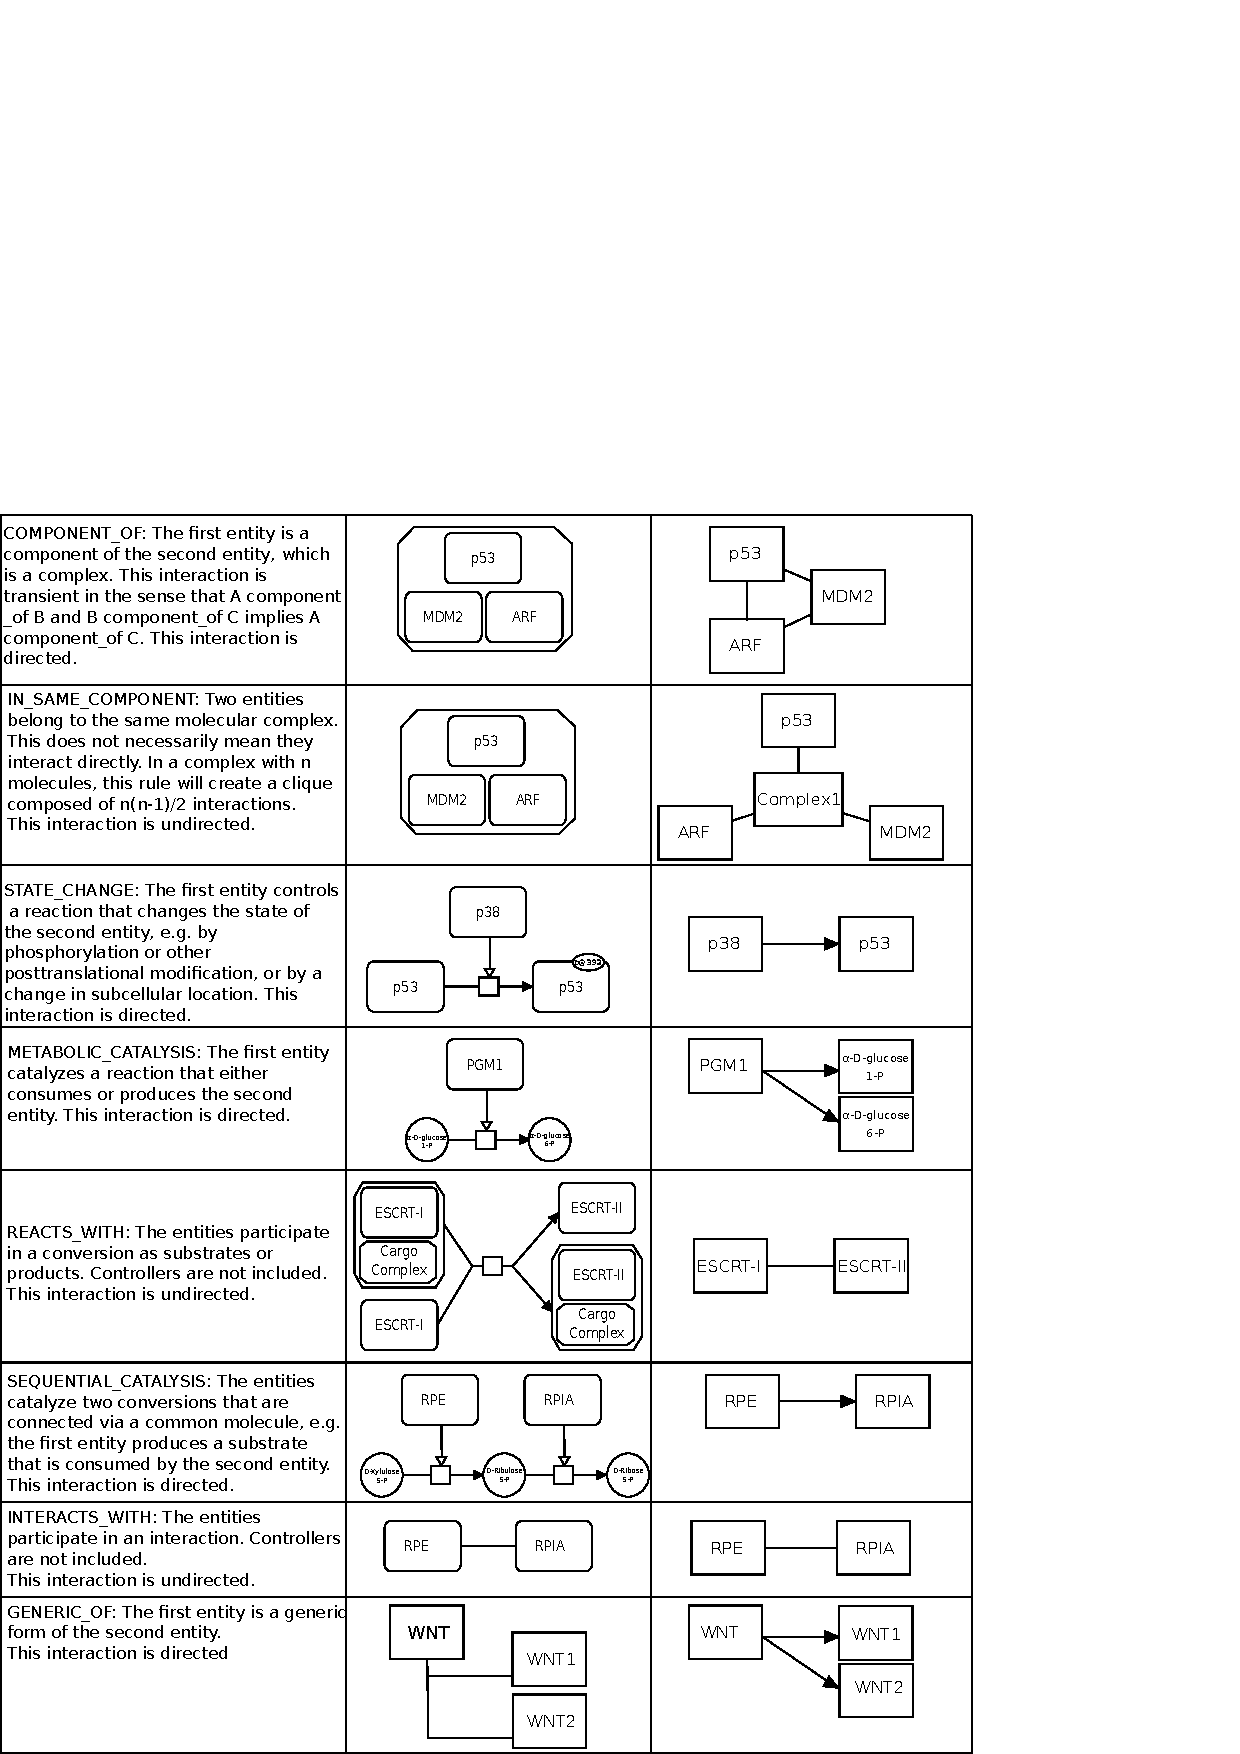
\includegraphics[width=\linewidth]{sifplain3.pdf}%
\caption{SIF rules: The left column is the recognized BioPAX pattern drawn in SBGN-PD, the right column is the resulting inferred SIF relationship(s).}
\label{fig:SIF}%
\end{figure*}

\subsection{Inference Rules}
Paxtools reduces BioPAX  to pairwise SIF relationships using a set of rules. Although this translation is lossy, SIF network remains useful for certain types of bioinformatics applications that require pairwise interaction input. The table below outlines these rules.
To export a BioPAX model to SIF, use the SimpleInteractionConverter class: 

\begin{javacode}
   SimpleInteractionConverter converter = 
   new SimpleInteractionConverter(new ControlRule());
   converter.writeInteractionsInSIF(level2, out);
\end{javacode}

Note the ControlRule object passed to the constructor. The constructor accepts a comma separated list of inference rules that are applied when binary interactions are requested. If not specified, all default binary interaction rules will be applied. You can also write your own rules by implementing the InteractionRule interface. 

\subsection{SIFNX Format}

SIFNX  is an extensible SIF-based format that allows users to customize the information extracted from the BioPAX model while keeping the simple binary network structure of SIF. You can use the same SimpleInteractionConverter class to export to SIFNX. For example, if you want to get the name of entities, their class, their external references and publications associated with interactions you can use:

\begin{javacode}
converter.writeInteractionsInSIFNX(model, 
     out, out, Arrays.asList("Entity/name","Entity/xref"),
    Arrays.asList("Entity/xref:PublicationXref"), true);
\end{javacode}

Parameters in this method represents the flexibility of SIFNX exporter. Model is the source model, and the two output streams are for writing out nodes and edges respectively. In this case, we opted to write both of them to the same stream. Next, two lists of strings define the path accessors to extract information for nodes and edges of the SIF. Finally, the last boolean parameter instructs converter to write the class of entity nodes to the export.

\subsection{PSI-MI (Proteomics Standards Initiative - Molecular Interaction)}
The PSI-MI format is a data exchange format for molecular interactions.  With help from the PSI-MI Developer Tools Library, the PSI-MI converter has the ability to create a BioPAX-L2 or BioPAX-L3 model from a PSI-MI Level 2.5 file.  For each EntrySet in the PSI-MI file, a BioPAX model is created.  For each Entry in the EntrySet, the converter creates a physicalInteraction (BioPAX-L2) or a MolecularInteraction (BioPAX-L3) for each interaction in the Entry.  Currently, genetic interactions are ignored.  For each Participant in the Interaction, the converter will create a sequenceParticipant (BioPAX-L2) or a SimplePhysicalEntity (BioPAX-L3).  The Participant's Interactor property determines the subclass of physical entity underlying the sequenceParticipant or SimplePhysicalEntity.  The converter will create a smallMolecule, dna, rna or protein class (BioPAX-L2) or SmallMolecule, Dna, Rna, or Protein class (BioPAX-L3) based on the type of Interactor.  This converter is also available using Paxtools from the command line.

\subsection{Gene Set Enrichment Analysis(GSEA)}
Paxtools  can create a Gene Matrix Transposed (*.gmt) file from a BioPAX-L3 model.  For each Pathway object in the model, the GSEA converter traverses all Protein objects in the Pathway and adds the RDF ID belonging to the first Xref returned by a call to Protein.getXref() to the gene set.  An optional external database name can be supplied to the converter, which would limit gene set membership to only those Protein objects that have an Xref to the external database.  The GSEA converter also has the ability to limit gene set membership to only those Protein objects that belong to the same species as the Pathway.  This converter is also available using Paxtools from the command line.

\subsection{Systems Biology Graph Notation - Process Description(SBGN-PD)}
Paxtools use libSBGN library to create SBGN -PD exports in SBGN-ML for BioPAX-L3 models. BioPAX-L3 to SBGN-PD conversion is an approximation because BioPAX-L3 is not always fully convertible to SBGN-PD. The main point of conflict is PhysicalEntity objects in BioPAX-L3 can define overlapping sets of pool of molecules, while EntityPoolNode (EPN) of SBGN-PD have to be disjoint. Paxtools creates an EPN for each PhysicalEntity as if they represent disjoint pools.
The following table is a summary of the conversion process.

\bigskip
\begin{center}
\footnotesize
\begin{tabular}{lp{10cm}l}
\toprule
BioPAX L3 component & Corresponding SBGN-PD glyph \\
\midrule
SimplePhysicalEntity &Glyph types "macromolecule", "simple chemical", "nucleic acid feature", and "unspecified entity" 
are used according to the type of the PhysicalEntity. \\
Conversion & A "process" glyph is created for each direction of the Conversion, i.e. two glyphs are created if the Conversion is reversible. "consumption" and "production" arcs are used to associate left and right participants, according to the direction.\\
Control & Controllers are linked with "catalysis", "stimulation", and "inhibition" arcs to the related process. When there are multiple Controller of the Control, they are connected with a logical "and" glyph. When the control has another control on itself, controls are connected with "and" glyph, and a "not" glyph is used after the second controller if the second control is negative. So the Control tree in BioPAX-L3 is represented with an "and" and "not" tree in SBGN-PD.\\
TemplateReaction & Similar to Conversion, a "process" glyph is created, but without the consumed participants. Instead, a "source and sink" glyph is created and linked with a "consumption" arc. \\
\bottomrule
\end{tabular}
\end{center}

The SBGN creation facility is implemented under the package org.biopax.paxtools.io.sbgn, and used as following:

\begin{javacode}
  //Create SBGN-PD and write to the given file
  L3ToSBGNPDConverter.writeSBGN(level3Model, "filename.sbgn");
\end{javacode}

\chapter{Running Graph Queries}

Paxtools provides several graph queries such as neighborhood, shortest + k paths, paths-in-between, common upstream, and common downstream, in the package org.biopax.paxtools.query. The algorithms used in the these queries are based on Dogrusoz et al.\cite{Dogrusoz2009}. Each query takes a source set (and sometimes also a target set) of BioPAX objects, the model, and several query parameters as input in their constructor. The run() method returns the result set of BioPAX objects.
To run graph queries, you can use the static methods of the class QueryExecuter:

\begin{javacode}
  Set<BioPAXElement> source = new HashSet<BioPAXElement>();
  // Add the related source PhysicalEntity 
  //(or children) objects to the  source set
  Collections.addAll(source, entity1, entity2, entity3);
  int limit = 2;
  // Direction can be upstream, downstream, or bothstream.
  Set<BioPAXElement> result = QueryExecuter.runNeighborhood(
   sourceSet, model,limit, Direction.BOTHSTREAM);
\end{javacode}

The query result will contain only the objects on the resulting paths. It will be a subgraph of the model, but it may not be a semantically consistent subgraph. For instance, consider the model : A, B, X are instances of PhysicalEntity, C is a Conversion, A is at the left of C, B is at the right of C, direction of C is left-to-right, and X is the positive Controller of C.
A neighborhood query with source X, limit 1, and towards downstream will retrieve the path X->C->B; however, this subgraph is not semantically complete. It contains a Conversion with a missing "left1" (in this case, an input). When the query result is detached from the model, for example if the query is being performed in a server, and the resulting graph is being sent to a visualization client, omitting A in the view will lead semantically incomplete view. In that case the user needs to use the Completer class to complete query result:

\begin{javacode}
Completer c = new Completer(
 SimpleEditorMap.get(BioPAXLevel.L3));
result = c.complete(result, model);
\end{javacode}

Now, the result set contains A because of C. This set can be safely cloned to get a valid BioPAX model.

QueryExecuter provides several methods for common graph queries:
\begin{itemize}
\item Neighborhood

Searches directed paths from and/or to the given source set of entities, in the specified search limit.

Parameters

\begin{itemize}
\item sourceSet: Set of source physical entities
\item model: Current model
\item limit: Search limit
\item direction:  Enum for search direction. Can be upstream, downstream, or bothstream.
\end{itemize}

\item GOI

GOI stands for graph-of-interest. This query retrieves the directed paths between the objects in the given source set. User gives a set of PhysicalEntity object and this query retrieves the graph connecting these entities.

Parameters

\begin{itemize}
\item sourceSet: Set of source physical entities
\item model: Current model
\item limit: Path length limit for the search
\end{itemize}


\item POI 

POI stands for paths-of-interest. Similar to GOI, but paths are searched from a source set, towards a target set. There are two types of search limit in this case. The first one is the normal limit, where you limit the length of the search paths by a value. The second is a shortest + k type limit, where the user specifies the value of k, and the actual limit becomes the length of the shortest path between sets plus k. The latter is useful when the user wants minimal connections between sets but does not know the length of the shortest path.

Parameters

\begin{itemize}
\item sourceSet: Source set of physical entities to start search
\item targetSet: Target set of objects to reach during the search
\item model: Current model
\item limitType: Whether to use a constant path length limit or a shortest+k limit
\item limit: Value of the limit. If limit type is shortest+k, then this represents k
\end{itemize}


\item PathsBetween 

This query is similar to GOI as it finds paths between a given source set of objects. The source set may contain Xref, EntityReference, and/or PhysicalEntity objects. They are automatically converted to sets of related PhysicalEntitiy objects to use as source in the query. The major difference here is that it avoids finding paths between PhysicalEntity objects that are associated with the same EntityReference, unless the user provides them explicitly in the source set. For instance, when the source set contains EntityReference of P53 protein, the query automatically finds all different modified versions of P53 in the model to use as seed in the query, but does not return paths between them. However, if a user provides different modification states of P53 in the source set, the query finds paths between them. The major use case of this query is the user has a set of entity references and wants to find paths connecting them.

Parameters

\begin{itemize}
\item sourceSet: Source set of xrefs, entity references, or physical entities
\item model: Current model
\item limit: Search limit
\end{itemize}


\item CommonStream

This query searches for the common upstream (common regulators) or common downstream (common targets) objects of the given source set. The source set should contain at least 2 elements.

Parameters

\begin{itemize}
\item sourceSet: Source set of physical entities
\item model: Current model
\item direction: Upstream or downstream
\item limit: Search limit
\end{itemize}


\item CommonStreamWithPOI

Common-stream query returns only the objects in the common upstream or downstream, but it does not include the paths leading to them. If a connected graph that contains both common objects and source objects is desired, then a POI query should be run between common objects and source objects. This method does it automatically.

Parameters

\begin{itemize}
\item sourceSet: Source set of physical entities
\item model: Current model
\item direction: Upstream or downstream
\item limit: Search limit
\end{itemize}
\end{itemize}

\chapter{Resources and Non-Java Access}

\section{Accessing Pathway Commons }
Pathway Commons (PC) is a convenient point of access to biological pathway information collected from BioPAX supporting public pathway databases. You can programmatically access PC using the pathwaycommons-client module. Currently there are two separate Pathway Commons clients implemented as part of the Paxtools under the org.biopax.paxtools.io.pathwayCommons package: PathwayCommonsIOHandler which interacts with the older PC WEB API and supports BioPAX Level 2; and PathwayCommons2Client which makes use of the newer PC WEB API and supports BioPAX Level 3. 

Using Pathway Commons Client you can search Pathway Commons, run graph queries in a bigger and more complete BioPAX graph or normalize your custom pathway using Pathway Commons services.

For example, here is a code snipplet which searches Pathway Commons 2 for the term "BRC*" restricting the results only to the BioPAX type Control and to the organism Homo sapiens; and then obtains these control reactions as a Paxtools model:

\begin{javacode}
  PathwayCommons2Client pc2 = new PathwayCommons2Client();
  pc2.setOrganisms(Collections.singleton("homo sapiens"));
  pc2.setType("Control");
  //Let's search for anything that starts with BRC
  SearchResponseType result = pc2.find("BRC*");
  HashSet<String> uris = new HashSet<String>();
  // For each search hit we got, get the uri for the 
 // resource at PC and add it to the set 
  for (SearchHitType hit : result.getSearchHit())
  {
   uris.add(hit.getUri());
  }
  //Create a model from this set of resources
  Model model = pc2.get(uris);
\end{javacode}


\section{Using Paxtools from the command line}
\begin{fullwidth}
Paxtools can be run as command line application.  Command line options are summarized below:

\begin{xmlcode}
merge file1 file2 output
toSif file1 output
toSifnx file1 outEdges outNodes prop1,prop2,...
validate path out [xml|html|biopax] [auto-fix] [normalize] [only-errors] [maxerrors=n]
integrate file1 file2 output
toLevel3 file1 output
fromPsimi level file1 output
toGSEA file1 output database crossSpeciesCheck
fetch file1 id1,id2,.. output
getNeighbors file1 id1,id2,.. output
\end{xmlcode}
 
If you have obtained Paxtools as a ("fat") JAR archive (e.g., a paxtools-YYYYMMDD.jar), then you can use the command line interface as the following:

\begin{xmlcode}
java -jar paxtools.jar --merge file1.owl file2.owl output.owl
\end{xmlcode}

For very large files you might want to increase jvm's memory:

\begin{xmlcode}
java -Xmx2048M -jar paxtools.jar --merge file1.owl file2.owl output.owl
\end{xmlcode}

You can also directly call the PaxtoolsMain class by:

\begin{xmlcode}
java -cp paxtools.jar org.biopax.paxtools.PaxtoolsMain --validate file.owl
\end{xmlcode}
\end{fullwidth}

\section{Using Paxtools from Python}

You can use JPype to control Paxtools from Python. You can download and install JPype from http://jpype.sourceforge.net/. Following example demonstrates how you can create a simple BioPAX model and write it out to a file using Python. 
\begin{fullwidth}
\begin{pythoncode}
from jpype import *
#call this to initialize use of Java
startJVM(getDefaultJVMPath(), "-ea", "-Xmx1g", "-Djava.class.path=paxtools.jar")

#get the paxtools root package as a shortcut
paxPkg = JPackage("org.biopax.paxtools")

#create a new BioPAX L3 factory
l3Factory = paxPkg.model.BioPAXLevel.L3.getDefaultFactory()

#create a new empty BioPAX model
model = l3Factory.createModel()

#define and set the xml base (URI prefix for elements we create)
xmlBase = "http://biopax.org/examples/pythonPaxtools#"
model.setXmlBase(xmlBase)

#get BioPAX classes (model interfaces); in this example: 
#Protein, CellularLocationVocabulary, UnificationXref:
proteinClass = java.lang.Class.forName(
 "org.biopax.paxtools.model.level3.Protein", 
 True, java.lang.ClassLoader.getSystemClassLoader())
cellularLocationCvClass = java.lang.Class.forName(
 "org.biopax.paxtools.model.level3.CellularLocationVocabulary", 
 True, java.lang.ClassLoader.getSystemClassLoader())
unificationXrefClass = java.lang.Class.forName( 
 "org.biopax.paxtools.model.level3.UnificationXref",
 True, java.lang.ClassLoader.getSystemClassLoader())

#create/add a couple of elements to the model
#Let's create a simple protein state using the factory method and unique identifier (URI)

protein = l3Factory.create(proteinClass, xmlBase + "protein1")
protein.addComment("python: created " + protein.getRDFId())

#And add it to the model
model.add(protein)

#step 3: set properties
protein.addAvailability("availability text")
cellLoc = l3Factory.create(
 cellularLocationCvClass, "http://identifiers.org/obo.go/GO:0005737")
model.add(cellLoc)
cellLoc.addComment("python: created " + cellLoc.getRDFId())
cellLoc.addTerm("cytoplasm")
protein.setCellularLocation(cellLoc)

#alternatively, one can create, set the id (URI), and add the element in one step
protein2 = model.addNew(proteinClass, xmlBase + "protein2")
protein2.addComment("created " + protein2.getRDFId())
\end{pythoncode}


\begin{pythoncode}
# let's add a unification xref to the CV
ux = model.addNew(unificationXrefClass, xmlBase + "XREF_GO_0005737")
ux.setDb("GO")
ux.setId("GO:0005737")
cellLoc.addXref(ux)

#export the model to a BioPAX OWL file
javaIO = JPackage("java.io")
io = paxPkg.io.SimpleIOHandler(paxPkg.model.BioPAXLevel.L3)
fileOS = javaIO.FileOutputStream("test.owl")
io.convertToOWL(model, fileOS)
fileOS.close()

#import a BioPAX model from the file
fileIS = javaIO.FileInputStream("test.owl")
model2 = io.convertFromOWL(fileIS)
fileIS.close()

#output to console
io.convertToOWL(model, java.lang.System.out)

#end use of jpype - docs say you can only do this once,
# so all java must be run before calling this
shutdownJVM() 
\end{pythoncode}
\end{fullwidth}

\chapter{Putting it all together}

Here is an example application that takes two or more protein names and queries/saves the neighborhood of each protein from Pathway Commons. It also queries the paths between these proteins, converts the resulting model to SIF and lists the publications that support each interaction in the final model. 

\begin{fullwidth}
\begin{javacode}
public class ProteinAnalyzer
{
 protected final static String outputPath = "files/";

 public static void main(String[] arg) throws IOException
 {
  /* Expects two or more protein names */
  if (arg.length < 2)
  {
   System.err.println(
     "Usage: ProteinAnalyzer protein1 protein2 [protein3 [protein4 [...]]]");
   System.exit(-1);
  }

  // This IO Handler will be used to export pathways in BioPAX format
  SimpleIOHandler ioHandler = new SimpleIOHandler();

  // Create the Pathway Commons client and configure it
  PathwayCommons2Client pc2 = new PathwayCommons2Client();
  // Search only for Proteins
  pc2.setType("Protein");
  // Restrict results to H. sapiens
  pc2.getOrganisms().add("homo sapiens");
  // Expand the graph query limit to get more results
  pc2.setGraphQueryLimit(2);

  // General set to collect ids of all matching protein
  Set<String> allProteinIds = new HashSet<String>();
\end{javacode}



\begin{javacode}
  for (String protein : arg)
  {
   // Search PC2 for the given protein name
   SearchResponseType searchResponse = pc2.find(protein);
   if (searchResponse.getTotalNumHits() < 1)
   {
    System.err.println("No results for protein:" + protein);
    System.exit(-1);
   }

   // Collect all ids associated to this search
   Set<String> ids = new HashSet<String>();
   for (SearchHitType searchHit : searchResponse.getSearchHit())
   {
    ids.add(searchHit.getUri());
   }

   // Also add all these ids to overall set
   allProteinIds.addAll(ids);

   // Query the neighborhood of this protein
   Model proteinNeighborhood = pc2.getNeighborhood(ids);
   // And export the resultant network in BioPAX format
   FileOutputStream fileStream = new FileOutputStream(
     outputPath + protein + ".owl");
   ioHandler.convertToOWL(proteinNeighborhood, fileStream);
   fileStream.close();
  }

  // Query the paths between all given proteins
  Model pathsBtwModel = pc2.getPathsBetween(allProteinIds);
  // Save the model in BioPAX format
  FileOutputStream pathsBtwFile = new FileOutputStream(
    outputPath + "pathBetween.owl");
  ioHandler.convertToOWL(pathsBtwModel, pathsBtwFile);
  pathsBtwFile.close();

  // Also save the model in Simple Interaction Format with all default rules
  SimpleInteractionConverter sifConverter = new SimpleInteractionConverter();
  FileOutputStream pathsBtwSIFFile = new FileOutputStream(
    outputPath + "pathBetween.sif");
  sifConverter.writeInteractionsInSIF(pathsBtwModel, pathsBtwSIFFile);
  pathsBtwSIFFile.close();

  // Now, get all interactions in the models to extract publication information
  for (Interaction interaction : pathsBtwModel.getObjects(Interaction.class))
  {
   // Print the name of the interaction
   System.out.println("* " + interaction.getDisplayName());
\end{javacode}



\begin{javacode}
   // Get all external references
   for (Xref xref : interaction.getXref())
   {
    String db = xref.getDb(),
      id = xref.getId(),
      url = "";

    // Convert PubMed ids to URLs for easy access
    if (db.equalsIgnoreCase("PubMed"))
     url = " (http://www.ncbi.nlm.nih.gov/pubmed/" + id + ")";

    // Print the external reference information
    System.out.println("\t" + xref.getDb() + ":" + xref.getId() + url);
   }}}}
\end{javacode}
\end{fullwidth}

\chapter{Frequently Asked Questions}

\textit{Q. When I convert BioPAX to simple interaction format file many relations contains unresolvable ids starting with  http://biopax.org/generated/group/.... How do I map this generated link to a known ID such as protein name or entrezID?}

A. Unresolvable URIs like this are used to represent groups that are either complexes, generics or generic complexes. Generics are typically families of proteins ( think WNT) that pathway databases captured as a group. A generic complex would be WNT-FRZ complex that maps to combinatorially many instances. Since in a SIF conversion nodes are entityReferences and complexes and some generics in BioPAX do not have entity references, without groups SIF conversion would be lossy or inaccurate. 

You can try toSifnx command to get external references as:

\begin{xmlcode}
java -Xmx1g -jar paxtools.jar toSifnx your_biopax_level3.owl 
 edges.txt nodes.txt  "EntityReference/xref:UnificationXref,
EntityReference/xref:RelationshipXref,Entity/xref:UnificationXref,
Entity/xref:RelationshipXref"  
"Interaction/dataSource/name,Interaction/xref:PublicationXref"
\end{xmlcode}

\textit{Q. I have encountered a conflict between jars and I get the following exception when I am reading BioPAX}

\begin{fullwidth}
\begin{xmlcode}
Exception in thread "main" org.biopax.paxtools.util.BioPaxIOException:
Unexpected element at start: 6
    at org.biopax.paxtools.io.SimpleIOHandler.readNameSpaces
\end{xmlcode}
\end{fullwidth}

A. This is a known problem caused by the StaX factory auto-discovery in JDK. You probably have two different stax implementations in your classpath. This problem also might happen under certain resource frameworks such as OSGi. For some discussion on this issue please see: http://code.cytoscape.org/redmine/issues/829.  Paxtools, in the future might allow different discovery solutions for different needs. As a temporary solution you can use the Jena based IO-handler.

\textit{Q. While reading a new BioPAX Level 3 model I am getting an error}

\begin{fullwidth}
\begin{xmlcode}
INFO Detected biopax namespace for level 2
INFO Using level: 2
ERROR org.biopax.paxtools.util.IllegalBioPAXArgumentException
	: No creation methods for name: SmallMolecule 
\end{xmlcode}
\end{fullwidth}
A. This sometimes happens with BioPAX files that contains both L2 and L3 namespaces confusing the auto level detection of the reader. Initialize your reader with the level explicitly:

\begin{javacode}
 JenaIOHandler jenaIOHandler = 
  new JenaIOHandler(
   new Level3FactoryImpl(), BioPAXLevel.L3);
\end{javacode}


\textit{Q. I am getting a lot of errors from the reader while reading BioPAX in the form of: ERROR org.biopax.paxtools.controller.PropertyEditor  - Failed to set value:.} 

A. This can happen either  due to non-standard usage or extensions of the BioPAX that is not in the specification. We constantly work with data providers to reduce such cases but you might still encounter them with an unvalidated BioPAX file. Examine the properties reported in the error log to determine what kind of information is being lost. In some cases these are not important for your usecase and you can ignore them. Otherwise try contacting the data provider to fix them.  Paxtools will provide support for extensions in the future releases.

\textit{Q. Is it possible --probably with loss of information-- to convert Level 3 files into Level 2?}
 
A. L3 contains significant changes compared to L2 and such a conversion would be quite lossy and problematic. Unfortunately, Paxtools can only convert L2 to L3.

\textit{Q. I am executing a paths-between query but the result is a BioPAX graph. I want to access the result paths separately. Where are the paths?}

A. All graph queries  return a graph which is the union of the queried paths, but they do not create the resultgraph by iterating over each result path. In most cases, there would be combinatorially many paths that are infeasible to enumerate.

\textit{Q. Why does Paxtools SBGN converter generates two process nodes for a reversible Conversion in the model when SBGN-PD can represent a reversible reaction with a single process node.}

A. This is due to a subtle semantic mismatch between SBGN-PD and BioPAX. In BioPAX a reversible BiochemicalReaction (subclass of Conversion) can have a directed Catalysis (left-to-right or right-to-left) based on the physiological context. If we use a single process node for the reversible reaction, we cannot show the direction of the Catalysis. If we use two process nodes, one for each direction, then we can associate the Catalysis only with the related process node. However, creation of two process nodes is only the default behavior and can be changed to single node using the "setUseTwoGlyphsForReversibleConversion" method if this is the user preference.

\textit{Q. I want to write an application that can handle both Level 2 and Level 3. Do I need to handle them separately?} 

A. This is a side effect of lack of backward compatibility between BioPAX Level 2 and 3 specification and it is not something we could directly address at the Paxtools level. BioPAX Level 3 was a major refactoring of the specification and it was impossible to maintain a common class hierarchy between 2 and 3. We have indeed a single class-base for Level 1 and Level 2 which are mostly backward compatible.,

To partially amend that situation we suggest all tool developers to upgrade the Level 2 models to Level 3 using the LevelUpgrader class and program to the Level 3 interfaces.  

The other option is to use the PropertyEditors and EditorMaps extensively. For example both BioPAX readers can read both level 2 and level 3. This requires a little bit more programming than the previous option but arguably offers a more robust solution. 

\textit{Q. I am confused by the statement "This syntactic validation does not include more detailed checking of semantics that is performed by the BioPAX validator." Which validation does what? Why is there a difference? Is the BioPAX validator not using Paxtools?}

A. The validator is built on Paxtools but is a separate project that includes a sophisticated rule defining and reporting system. Paxtools limits itself to so-called \textit{invariants} of the BioPAX specification, namely, RDF well-formedness, domain and range restrictions, bidirectional links, and redundancies. When these constraints are violated Paxtools fails-fast  by throwing an exception. Checking additional semantics and best practices such as using proper controlled vocabularies or ensuring that a transport reaction has at least one substrate that changes its subcellular location as result of the reaction is left to the validator. There are no technical reasons for not including validation rules within Paxtools - in fact historically some of the current validator rules were a part of Paxtools. We quickly found out, however, that this was severely restricting our user base as they were using Paxtools and BioPAX in ways that we have not imagined. As a result we moved all of these optional constraints to the validator and built a system where users can activate and deactivate which rules are to be checked and how they are going to be reported( e.g. warnings vs. errors). 

\textit{Q. Why are level2 model interfaces are not in CamelCase?}

A.Class names of model interfaces strictly mirrors BioPAX specification and level 2 was specified using the LISP syntax.  We decided to copy the case directly from the specification to avoid any confusion.  In Level 3, BioPAX specification was migrated to CamelCase to amend that based on our input. All other classes in Paxtools strictly follow CamelCase and Java naming conventions. 

\textit{Q. What happens to the additional properties that are not a part of BioPAX specification? If I define new properties or classes, can Paxtools read and write them?}

A. The short answer is no - they are lost when you read them with Paxtools. The long answer is this is an important feature that we wanted to add but it turns out to be surprisingly difficult. Adding a simple custom property can be done relatively easily by adding a HashMap<key,Set> to every object but things get complicated when trying to implement more advanced OWL properties such as subproperties, symmetric and transitive properties. We felt that it would be inconsistent to offer a facility to read arbitrary extensions of the BioPAX specification in the OWL file but limit ourselves to only simple properties. We have an early alpha implementation that did not make the cut for the latest release. We will include this facility in the future releases.

On the other hand, we believe that extending the library in the traditional sense by extending the classes is in fact very easy. In fact Paxtools were designed right from the start to enable such an extension by implementing a factory pattern for object creation and PropertyEditors for reading/writing properties.

\textit{Q.  While exporting to SBGN-ML, I wonder why two process glyphs are created when a Conversion is reversible as it can be presented with one process glyph only as illustrated in \url{http://www.sbgn.org/Symbols/consumption_production_reversible}?}

A. This choice is made because of the BioPAX structure. In BioPAX, a reversible BiochemicalReaction can have a Catalysis with a specific direction. If we draw one process glyph for the reversible BiochemicalReaction, then we cannot show the direction of the Catalysis. In the two process glyphs case, the Catalysis will point to the related process glyph only. However, we realize that some users may opt for a reversible process glyph even though they can not visualize the Catalysis direction, and we now provide this as an option in the exporter. 


\chapter{A few last words...}
\section{Acknowledgements}
We would like to thank Ethan Cerami, Istemi Bahceci, Nadia Anwar, Ugur Dogrusoz, Ruth Isserlin, Guanming Wu, Suzanne Mercer Paley, Sasha Tkachev, Carl Schaefer, Takeshi Yoneki, Anushya Muruganujan, Sarala Wimalaratne, Nick Juty, Oliver Ruebenacker, Andrea Splendiani, Allan Ruttenberg, Martijn Van Iersel, Akira Funahashi, Logan Webb, Ranjani Ramakrishnan, Rebecca Tang, Rex Dwyer, Adem Bilican, Afshin Sadeghi, Alejandra Lopez Fuentes, Allyson Lister, Anatoly Sorokin, Anatoly Ulyanov, Anna Bauer-Mehren, Ashok Reddy Dinasarapu, Augustin Luna, Micheal Blinov, Brian Saunders, Brian Turner, Bruno Aranda, Jeff Buchoff, David Dunkley, Peter D'Eustachio, Esat Belviranli, Farzana Kazi, Francois Le Fevre, Fong Chun Chan, Hester Stekelenburg, Irma Martinez-Flores, Jean-Baptiste Pettit, Jing Wang, Julie Sullivan, Karin Brauer, Josh Stuart, Julio Saez-Rodriguez, Olivier Gevaert, Paul Shannon, Peter Karp, Pradeep Kumar Sreenivasaiah, Ricardo Usbeck, Sai Lakshmi Subramanian, Stan Dong, Samer Hanoudi, Sarah Boyd, Ufuk Kirik, Zhihua Li, Zhenjun Hu and other members of the  BioPAX community for their contributions and feedback.  
\section{Get Involved}
\begin{fullwidth}
Paxtools is open source software and we welcome all contributions.  Get involved! 
\begin{itemize}
\item Use Paxtools and report issues and feature requests.  : \url{http://biopax.sourceforge.net/paxtools/issue-tracking.html}
\item Try your hand at fixing bugs and implementing requests .
\item Respond to questions by other users at biopax-paxtools :  \url{http://lists.sourceforge.net/lists/listinfo/biopax-paxtools}
\item Improve this documentation:  \url{http://sourceforge.net/p/biopax/paxtools/ci/default/tree/src/main/etc/}
\item Spread the word. Let other people know about BioPAX and Paxtools. : \url{http://biopax.org} 
\end{itemize}
\end{fullwidth}

\bibliographystyle{emek}
\nobibliography{paxtools}

\end{document}
